\section{Problem Statement} \label{sec:Formulation}
\hl{We assume that we are given a corpus $\mathscr{C}$ of annotated resources, where each resource is associated with a variable number of tags}. The corpus contains:
\begin{itemize}
\item \hl{Set of resources: $\mathcal{R}=\left\{ r_l \right\}$ where $l=1$ to $\mid\mathscr{C}\mid$}
\item Set of tags in the corpus: $\mathcal{T}=\left\{t_j \right\}$ where $j=1$ to $N$ 
\item \hl{A binary tag association matrix $\mathcal{B}$. $\mathcal{B}(r,j)=1$ if tag $t_j$ is associated with resources $r$, and $0$ otherwise. }
\end{itemize}
We define an ontological tag tree as an undirected weighted tree on the set of tags $\mathcal{T}$. This implies that the tag tree is connected and has no simple cycles. The task is to arrange the set of tags $\mathcal{T}$ in an ontological tag tree. 


\section{Construction of Ontological Tag Tree}
\label{sec:ConstructionTree}
In order to construct the tag tree, we propose an approach that starts with a preliminary tag tree obtained using the semantics encoded in WordNet hierarchy. We follow this by a corpus statistics based tag tree refinement.

Construction of the WordNet based preliminary tree is described below. 

\subsection{Constructing WordNet-based Preliminary Tag Tree}
\label{sec:WordNetGraph}
We follow the approach outlined in \cite{WordnetHierarchyConstruct} to derive the semantic relations between the set of tags $\mathcal{T}$. This is done in two stages. In the first stage, disambiguation for the meaning of the tags is done by selecting the most popular concept (synonym set, or synset) for every tag. For example a tag ``turkey" can be mapped to the bird, or the country. In WordNet, since the synset corresponding to Turkey, the bird, has a higher frequency count than the synset corresponding to the Republic of Turkey, the former synset would be selected to map to the tag ``turkey". Then in the second stage, in order to find the relationships between different tags, all links between the mapped concepts are found through the WordNet hierarchy for semantic relationships ``is-a" or ``part-of". Since we are only interested in a tag tree which has undirected edges between the tags, we ignore the directions of the edges in the obtained hierarchy, which could otherwise help distinguish more generic concepts or tags from more specific ones. 

\indent The resulting undirected graph in general has cycles and is usually disconnected, forming disjoint clusters of tags. In order to construct a tree from the above undirected graph, we first break the cycles and then connect disjoint segments in a greedy manner using inter-tag semantic distances as obtained from WordNet Library \cite{RitaLibraryWordNet}. The semantic distance between two synsets in WordNet is defined as: 
%We follow the approach outlined in \cite{WordnetHierarchyConstruct} to construct a WordNet-based hierarchy for the set of tags $\mathcal{T}$. This is done in two stages. In the first stage, disambiguation for the meaning of the tags is done by selecting the most popular concept (synset) for every tag. Then, in order to find the relationships between different keywords, all links between the mapped concepts are found through the WordNet hierarchy for semantic relationships such as "is-a" or "part-of". Since we are only interested in a tag tree which has undirected edges between the tags, we ignore the directions of the edges in the obtained hierarchy, which could otherwise help distinguish more generic concepts or tags from more specific ones. 
%The resulting undirected graph in general has cycles and is usually disconnected, forming disjoint clusters of tags. To address these issues, we utilize a heuristic to construct a tree from the above undirected graph. Towards this, we utilize inter-tag distances from the WordNet Library \cite{RitaLibraryWordNet} defined as:
\begin{equation}
\frac{\text{ MHP }}{\text{HPR + MHP }}
%\frac{\text{ Minimum hops to common parent }}{\text{Hops from common parent to Root + Minimum hops to common parent}}
\label{eq:ritaDistance} 
\end{equation} 
where 
MHP:= Minimum hops to common parent, and 
HPR:= Hops from common parent to Root of hierarchy. We define the \textbf{semantic distance} between tags $i$ and $j$ as the semantic distance between the respective WordNet synsets. 
%Semantic similarity between tags $i$ and $j$ is defined as ($1-$ Semantic distance between $i$ and $j$).
The steps of the procedure for obtaining a preliminary ontological tag tree starting from WordNet hierarchy are summarized in Algorithm~\ref{alg:WordNetSTAlgo}, which returns a tree over the set of tags $\mathcal{T}$. 

\begin{algorithm}
\fontsize{8pt}{1em}\selectfont
\caption{Constructing Preliminary Tag Tree using WordNet hierarchy} 
\label{alg:WordNetSTAlgo} 
\textbf{Input:} \\
$\cdot$ WordNet based hierarchy $\mathcal{H_T}$ for given set of tags $\mathcal{T}$ representing semantic relationships such as ``is-a" or ``part-of". $\mathcal{H_T}$ is directed graph and can be disconnected. \\ 
$\cdot$ Pair-wise semantic distances for tags in $\mathcal{T}$ from (\ref{eq:ritaDistance})\\
\textbf{Breaking cycles:} \\
Obtain $H_{undirected}$ as the undirected version of $\mathcal{H_T}$ \\
\textbf{Loop While} cycles exist in $H_{undirected}$ \\
\hspace*{5mm} $\cdot$ Find one cycle in $H_{undirected}$. $E_{cycle}$=edges in the \\
\hspace*{5mm} \; obtained cycle \\
\hspace*{5mm} $\cdot$ Remove the edge $e \in E_{cycle}$ with largest distance (\ref{eq:ritaDistance}) \\
\hspace*{5mm}  \; from $H_{undirected}$ \\
\textbf{EndWhile} \\
\textbf{Connecting disjoint components in $H_{undirected}$:} \\ 
\textbf{Loop While}  $H_{undirected}$ is disconnected \\
\hspace*{5mm} $\cdot$ Obtain pair-wise distances between tags from (\ref{eq:ritaDistance}) \\
\hspace*{5mm} $\cdot$ Set distances between tags in same component, to $\infty$ \\
\hspace*{5mm} $\cdot$ Connect tags with least distance. These will form edges \\
\hspace*{5mm} between the disjoint components. \\
\textbf{EndWhile}. \textbf{Output:}  tree $T_W$ 
\end{algorithm}
Once the preliminary tag tree based on WordNet, $T_W$, is constructed as described, we refine it using a data driven approach based on the co-occurrence statistics of the tags. We describe this below. 
\subsection{Co-occurrence based Tag Tree Refinement}
\label{sec:refinement}
The preliminary tag tree is refined by accounting for those tags that strongly co-occur in the corpus but are not linked in the WordNet based tag tree. To achieve this, we first define the similarity score of two tags using {\bf {\em Jaccard Similarity}}:
\begin{definition}
{\bf [Jaccard Similarity]}: The Jaccard Similarity $J(s_1, s_2)$ between two sets $s_1, s_2$ is defined to be equal to
\begin{equation} 
\frac{|s_1 \cap s_2|}{|s_1 \cup s_2|}.
\label{eq:jaccard}
\end{equation}
\end{definition}

\hl{Let $\mathcal{T}=\{t_j\}_{j=1}^N$ be the set of tags and $\mathcal{R} = \{r_l\}_{l=1}^{\mid\mathscr{C}\mid}$ be the set of resources}. For each tag $t_j$ we construct the set $s_j = \{ r : r \in \mathcal{R} \mbox{ and } \mathcal{B}(r,j)=1 \}$. Let $J_{\mathcal{T}}$ be an $N \times N$ matrix such that $J_{\mathcal{T}}(i,j) = J(s_i, s_j)$. We will call $J_{\mathcal{T}}$ the {\bf Jaccard Matrix} of $\mathcal{T}$.

We augment the preliminary tag tree based on WordNet, $T_W$, to construct a \textbf{Similarity Graph} as follows. We construct the graph with vertex set $V = \{v_1,\ldots, v_N\}$ where the $v_j$ corresponds to the tag $t_j$. We start with $T_W$, which is a tree on $V$ constructed using WordNet as described in Algorithm~\ref{alg:WordNetSTAlgo}. Additionally, given a threshold $\tau$, $0\leq \tau \leq 1$, we join $v_i, v_j$ with an edge iff $J_{\mathcal{T}}(i,j) \geq \tau$, and the edge weight of edge $(v_i,v_j)$ is set to be $J_{\mathcal{T}}(i,j)$.  We call the resulting graph $\mathcal{G_T}$, the {\bf Similarity Graph} of $\mathcal{T}$ since it captures the tree based on semantic similarity, and additional edges based on corpus based jaccard similarity. Fig.~\ref{fig:sim} shows an illustrative example for obtaining Similarity Graph based on a threshold $\tau$.
\begin{figure}[h]
\centering
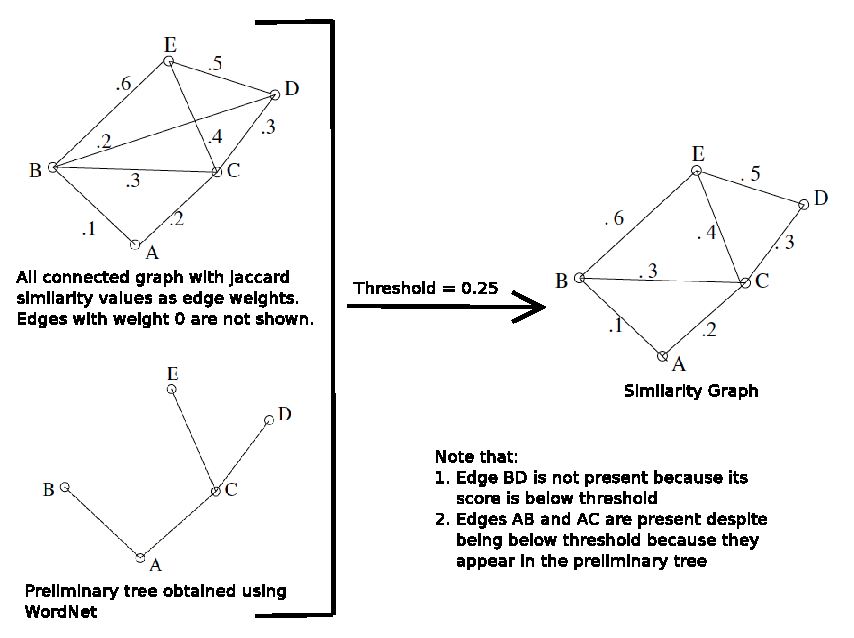
\includegraphics[width=0.8\linewidth]{TagTree/CreatingSimGraph}
\caption{Building the Similarity Graph for threshold $\tau$=0.25} 
\label{fig:sim}
\end{figure}
%\subsection{Objective Function} \label{subsec:objfunction}
Given the similarity graph $\mathcal{G_T}$, the objective of the refinement stage is to find a tree in the space of spanning trees of the similarity graph $\mathcal{G_T}$ which minimizes a defined objective function. Below we define and motivate two different objective functions based on corpus statistics, for tag tree construction. 
\begin{enumerate}
\item \textbf{Weighted Average Hops (WAH)}: 
\begin{equation}
\; \sum_i\sum_{j, j < i}{J_{\mathcal{T}}(i,j)d_{i,j}} , 
\label{eq:ObjFnWeightedHops}
\end{equation}
where $d_{i,j}$ represents the number of hops between tag $t_i$ and tag $t_j$ in the tag tree. The motivation for such a score is that it is lower when tags $i$ and $j$ with high $J_{\mathcal{T}}(i,j)$ are separated by fewer hops as compared to tags with low $J_{\mathcal{T}}(i,j)$. \hl{The above objective function is equal to the sum of the pair-wise hops between all pairs of tags weighted by the corresponding Jaccard similarity {$J_{\mathcal{T}}(i,j)$}. Dividing the sum by 
$\sum_{i,j < i}{J_{\mathcal{T}}(i,j)}$ would be equal to the weighted average number of pair-wise hops where the weights are normalized Jaccard similarities. Since the value $\sum_{i,j <  i} {J_{\mathcal{T}}(i,j)}$ is a constant for a given set of tags {$\mathcal{T}$}, we have removed the scaling factor from the objective function. }
For a general graph $\mathcal{G_T}$, the problem of minimizing the weighted average number of hops has been established to be an NP hard problem \cite{garey1979computers}.  
\item \textbf{Similarity Approximation (SA)}: 
\begin{equation}
\; \sum_i\sum_{j, j < i}{w_{i,j}\mid J_{\mathcal{T}}(i,j) - S_T{(i,j)}} \mid  , \\
\label{eq:ObjFnSimApprox}
\end{equation}
where $S_T{(i,j)}$ represents the similarity between tags $t_i$ and $t_j$ estimated using tag tree $T$. A very close problem is that of approximating a given distance matrix through spanning trees, which has been established to be NP hard~\cite{eckhardt2005combinatorial}. The objective function in~(\ref{eq:ObjFnSimApprox}) is the weighted L1 norm of the difference between the Jaccard Matrix $J_{\mathcal{T}}$ and the \textbf{Estimated Similarity Matrix} $S_T$. \hl{The weights $w_{i,j}$ are taken to be the co-occurrence counts of tags $t_i$ and $t_j$ and are useful to establish relative importances between different pairs of tags in the objective function}. While $S_T{(i,j)}$ can be calculated in several ways for a given tag tree $T$, we define $S_T{(i,j)}$  as 
\begin{equation}
S_T{(i,j)} = \prod_{e \in \mathfrak{P}_{i,j}}{S(e)}  , \\
\label{eq:ProdSimSimilarityCalculate}
\end{equation}
where $\mathfrak{P}_{i,j}$ is the path in tag tree $T$ connecting tags $t_i$ and $t_j$ and $S(e)$ is equal to the Jaccard similarity between the tags that edge $e$ connects. Such a definition for $S_T{(i,j)}$  ensures that it lies between 0 and 1 and no rescaling is required in order to compare $S_T{(i,j)}$  values with $J_{\mathcal{T}}(i,j)$.
\end{enumerate}
\hl{Note that the trees in ({\ref{eq:ObjFnWeightedHops}}) and ({\ref{eq:ObjFnSimApprox}}) are constrained to be spanning trees over the Similarity Graph $\mathcal{G_T}$. }The local search based approach to minimize either of the above objective functions is described next. 
\vspace{-0.12in}